\chapter{コサイン類似度を用いたi-vectorの性質の調査}
発話間のi-vectorのコサイン類似度を算出し、発話の長さごとに同一話者の発話間の場合と異なる話者の場合に分けてヒストグラムに表し、性質を調査した。
\section{使用する音声データ}
\subsection{UBMモデルの学習に使用する音声データ}
UBMの作成には大量の不特定話者の音声データが必要である。本研究では、学習データとして、読み上げ音声\cite{ATR}(50発話×男女各110人分)を使用した。
\subsection{検証に用いる音声データ}
評価データとしてニュース番組の音声データ13個を用いる。各音声データには、事前に人手で4種類(音楽、音声、雑音、無音)の音源ラベルが付与されている。「音声」の音源ラベルが付与された区間においては、更に発話者の情報が付与されている。また「音声」の音源ラベルをもとに対象の音声データから発話区間を抽出し、それを一発話とした。\par
表\ref{val_detail}に検証に用いるデータの詳細を示す。

\begin{table}[htb]
  \begin{center}
  \label{val_detail}
    \caption{検証用データの詳細}
    \begin{tabular}{|c||c|c|c|} \hline
      データID & 収録時間 & 話者数 & 全発話数 \\ \hline
      ニュースA & 30分3秒 & 20 & 337 \\ \hline
      ニュースB & 30分3秒 & 31 & 312\\ \hline
      ニュースC & 30分3秒 & 21 & 324 \\ \hline
      ニュースD & 30分4秒 & 20 & 324\\ \hline
      ニュースE & 20分3秒 & 13 & 159\\ \hline
      ニュースF & 30分3秒 & 22 & 343\\ \hline
      ニュースG & 30分4秒 & 22 & 313\\ \hline
      ニュースH & 30分4秒 & 20 & 315\\ \hline
      ニュースI & 30分4秒 & 17 & 321\\ \hline
      ニュースJ & 30分4秒 & 16 & 337\\ \hline
      ニュースK & 30分4秒 & 20 & 363\\ \hline
      ニュースL & 30分4秒 & 26 & 345\\ \hline
      ニュースM & 30分4秒 & 26 & 314\\ \hline
    \end{tabular}
  \end{center}
\end{table}


\section{コサイン類似度の算出条件}
対象の音声データからある発話を取り出し、それ以外の発話とのi-vectorのコサイン類似度を算出する。それを同一話者の発話間の場合と異なる話者の発話間の2つの場合に分けてヒストグラムに表し、コサイン類似度の性質の調査を行った。\par
i-vectorの抽出に使用するUBMモデルの学習には読み上げ音声\cite{ATR}を使用し、発話から抽出する音響特徴パラメータを表\ref{iv_feature}に示す。また混合数は32とした。

\begin{table}[htb]
  \begin{center}
    \caption{使用する音響特徴パラメータ}
    \label{iv_feature}
    \begin{tabular}{|c||c|} \hline
      特徴量 & 次元数\\ \hline
      MFCC & 19  \\ \hline
      POW & 1  \\ \hline
      $\Delta$MFCC & 19 \\ \hline
      $\Delta$POW & 1 \\ \hline
      $\Delta\Delta$MFCC & 19 \\ \hline
      $\Delta\Delta$POW & 1 \\ \hline
      計 & 60 \\ \hline
    \end{tabular}
  \end{center}
\end{table}

本研究では、音響特徴量のひとつとしてメル周波数ケプストラム係数(MFCC)を用いる。メル周波数ケプストラム係数(Mel - Frequency Cepstrum Coefficient : MFCC)とは、メル周波数という人間の音の高低に対する感覚尺度を考慮した特徴量であり、音声スペクトルから係数スペクトルを抽出したものである。これは一般的に、音声の特徴を抽出するパラメータとして用いられる。[5]

\section{比較的長い音声データから抽出したi-vectorの性質}
本節では、比較的長い音声データとして、5秒間の音声データからi-vectorを抽出した。その結果、図\ref{fig:iv_same_long}より、同一話者の発話間の場合はコサイン類似度が高い値に多く分布し、図\ref{fig:iv_other_long}より、異なる話者の発話間の場合はコサイン類似度が全体的に分布していることが分かる。\par
これより、比較的長い音声データでは、コサイン類似度の値が高いほど、i-vectorを照合した発話の話者が同一の話者である確率が高いということが分かる。

\begin{figure}[htb]
  \begin{center}
    \includegraphics{../../image/image_dnn.eps}
  \end{center}
  \caption{比較的長い音声データから抽出した同一話者間のi-vectorのコサイン類似度}
  \label{fig:iv_same_long}
\end{figure}

\begin{figure}[htb]
  \begin{center}
    \includegraphics{../../image/image_dnn.eps}
  \end{center}
  \caption{比較的長い音声データから抽出した異なる話者間のi-vectorのコサイン類似度}
  \label{fig:iv_other_long}
\end{figure}

\section{非常に短い音声データから抽出したi-vectorの性質}
本節では、非常に音声データとして、0.3秒間の音声データからi-vectorを抽出した。その結果を図\ref{fig:iv_same_short}と図\ref{fig:iv_other_short}に示す。\par

\begin{figure}[htb]
  \begin{center}
    \includegraphics{../../image/image_dnn.eps}
  \end{center}
  \caption{非常に短い音声データから抽出した同一話者間のi-vectorのコサイン類似度}
  \label{fig:iv_same_short}
\end{figure}

\begin{figure}[htb]
  \begin{center}
    \includegraphics{../../image/image_dnn.eps}
  \end{center}
  \caption{非常に短い音声データから抽出した異なる話者間のi-vectorのコサイン類似度}
  \label{fig:iv_other_short}
\end{figure}

これより、非常に短い音声データから抽出したi-vectorは同一話者であっても必ずコサイン類似度が1に近づくということはなく、十分に話者の特徴を抽出できていないことが示されている。
